\documentclass{article}

% Language setting
% Replace `english' with e.g. `spanish' to change the document language
\usepackage[english]{babel}
\usepackage{fontawesome5}
\usepackage{listings}
\usepackage{tcolorbox} % For colored and framed text blocks
\usepackage{tabularx}
\usepackage{caption}
\usepackage{tikz}
\captionsetup[table]{skip=0pt,singlelinecheck=off}

\usepackage{fancyhdr}
\pagestyle{fancy}
\fancyhf{}
\fancyfoot[R]{\thepage}

% Define a custom environment for code blocks
\tcbuselibrary{listingsutf8} % Allows for verbatim-like content inside tcolorbox


% Monospace code box settings
\newtcolorbox{codeblock}{
    coltitle=black,
    boxrule=0mm,
    sharp corners
}


\usepackage{exsheets}
\SetupExSheets{
  headings = block-subtitle ,
  subtitle-format = \bfseries % default is \itshape
}
\RenewQuSolPair{question}[name=\faClipboard[regular] Exercise]{solution}

% Set page size and margins
% Replace `letterpaper' with `a4paper' for UK/EU standard size
\usepackage[letterpaper,top=2cm,bottom=2cm,left=3cm,right=3cm,marginparwidth=1.75cm]{geometry}

% Useful packages
\usepackage{amsmath}
\usepackage{graphicx}
\usepackage[colorlinks=true, allcolors=blue]{hyperref}

\setlength\parindent{0pt} % no indent for new paragraphs
\setlength{\parskip}{16pt}

\title{BIO334 - von Mering}
\author{04 - Phylogenetic Trees - Part 1 (Distance-based methods)}

\date{2025}
\begin{document}
\maketitle
\vspace{-10pt}
\begin{question}[subtitle = Calculating sequence distances from multiple alignments]
    In the first two exercises, you will have (nearly) no need of your computer, but all the more for paper and pencil: we will try to obtain a \textbf{UPGMA} (\textbf{U}nweighted \textbf{P}air \textbf{G}roup \textbf{M}ethod with \textbf{A}rithmetic \textbf{M}ean) tree from a multiple sequence alignment with the bottom-up approach.
    
    In the previous lecture, you used different tools to produce multiple alignments of representatives of the \textbf{MFS-1} domain, based on a protein isolated from a 1000-year-old tooth plaque (dental calculus). Now, we will try to build phylogenetic trees to further investigate the evolutionary relationship between those different proteins. We will work with the following subset of proteins from the multiple alignment exercises (BLAST hits to the query protein MFS-1 domain, aligned with Clustal Omega):
    \begin{codeblock}
        \begin{center}
            \texttt{Protein\_Q  GDRVG RKFII WFSIL GTAPF ALWLP YAD-A DTTAI LVILI GFIIS SAFAS}\\
            \texttt{Protein\_A  GDRVG RKFII WFSIL GAAPF ALWLP YAD-A QTTAI LIVLI GFIIS SAFAS}\\
            \texttt{Protein\_B  GDKVG RKYII WFSVL GVAPF TMLLP YAS-L EWTGI LIVII GLILS SAFPS}\\
            \texttt{Protein\_C  GDRFG RKYVI WFSIL GTAPF ALMLP YAN-L FWTGV LIVPI GMILA SAFSA}\\
            \texttt{Protein\_D  GDRIG RKYVI WGSIL GVAPF TLILP YAS-L YWTGI LTVII GFILA SAFSA} 
        \end{center}
    \end{codeblock}

   First, we need to obtain a measure of \textit{evolutionary distance} between these five proteins by calculating \textit{sequence similarity} between them. For now, we will use a simple "similarity" measure: the ratio of shared vs. not-shared characters per position between the two sequences. This is also called the \textit{Jaccard} index \textbf{J}:
    \begin{equation}
        J(A,B) = \frac{|A\cap B|}{|A\cup B|}
    \end{equation}
    \small{\textit{Note: $A\cap B$ is the intersection between the two sequences, i.e. the positions where the “character” between sequence A and B is equal (intersection) while $A\cup B$ the union, i.e. all the positions. We consider the dash (-,gap character) in the alignment as a position}}

    Using the Jaccard Index we can define a measure of distance, i.e. the larger the more distant:
    \begin{equation}
        d_j(A,B) = 1- J(A,B)
    \end{equation}
    Calculate the pairwise Jaccard distances and fill in the following distance matrix:
    \begin{table}[!h]
        \centering
        \caption*{Distance matrix D}
        \label{tab:my-table}
        \begin{tabularx}{1\textwidth} {
            | >{\centering\arraybackslash}X 
            | >{\centering\arraybackslash}X 
            | >{\centering\arraybackslash}X 
            | >{\centering\arraybackslash}X
            | >{\centering\arraybackslash}X
            | >{\centering\arraybackslash}X |
        }
        \hline
        \textbf{d$_j$} & \textbf{Q}   & \textbf{A} & \textbf{B} & \textbf{C} & \textbf{D} \\ \hline
        \textbf{Q}     & 0.0 &   &   &   &   \\ \hline
        \textbf{A}     &     &   &   &   &   \\ \hline
        \textbf{B}     &     &   &   &   &   \\ \hline
        \textbf{C}     &     &   &   &   &   \\ \hline
        \textbf{D}     &     &   &   &   &   \\ \hline
        \end{tabularx}
    \end{table}
    
    \pagebreak
    Now think for a moment about the following questions:
    \begin{enumerate}
        \item What is the computational complexity of distance matrix calculations: with increasing number of proteins, how will the run time increase? Assuming that the distance matrix for 1000 proteins takes 1s to compute, how long will it (roughly) take for 10.000, 100.000, 1.000.000, 10$^9$ proteins?
        \item As said before, the Jaccard index is quite simple, and probably provides a very inaccurate estimate of the evolutionary distance between two sequences. In which ways could the distance calculation be modified to provide a more realistic estimate of the “true” underlying evolutionary processes? Which parameters could have the strongest influence on the accuracy of any distance estimate?
        \item Protein sequences and nucleotide sequences (DNA/RNA) provide similar yet distinct types of information. What are the most striking differences between the two with regard to the calculation of evolutionary distances? For which kinds of problems or studies would you prefer one or the other, and why?
    \end{enumerate}
    *\underline{Optional Task}
    \begin{enumerate}
        \item Can you write a Python script to compute the pairwise Jaccard distance J matrix for any number of sequences? You can use the sequences in the FASTA file \texttt{ex1\_sequences.fa} to test your script.
    \end{enumerate}
\end{question}
\pagebreak
\begin{question}[subtitle = Exploring the UPGMA Algorithm]

    Based on the $5 \times 5$ distance matrix D you computed above, we will make a phylogenetic tree relating the proteins by using the UPGMA (\textbf{U}nweighted \textbf{P}air \textbf{G}roup \textbf{M}ethod with \textbf{A}rithmetic \textbf{M}ean) algorithm. We’ll provide a step-by-step walkthrough here and if you like to dig deeper on the topic, you can check \href{https://en.wikipedia.org/wiki/UPGMA}{UPGMA on Wikipedia}. A very nice and interactive explanation of the algorithm is also \href{http://www.slimsuite.unsw.edu.au/teaching/upgma/}{online}.

    \textbf{Overview of the algorithm}

    We start with an unstructured, unrooted phylogenetic tree in which n sequences represent n leaves, while we do not know their appropriate connections and branch lengths. Given a pairwise distance matrix of size $n \times n$, the related $n \times n$ D matrix of pairwise sequence relations (distances) can be computed. Based on the D matrix, the two most related leaves are joined at a tree node, and their respective distances from this node (the branch lengths) are computed. Subsequently, a new distance matrix is computed by calculating pairwise distances of all remaining elements to the newly formed node (the resulting new distance matrix is of size $(n-1) \times (n-1)$). This procedure is repeated until all relations are resolved.

    \textbf{1. Choose first two elements (proteins) to join}

    Looking at the distance matrix D (the one you computed above), choose the two closest proteins (in terms of sequence distance) and create a new distance matrix D2. You will see that the closest two proteins in terms of J distance from matrix D are in fact proteins Q and A, so we will make a new "node" (cluster) named "QA" out of these two proteins and compute a new matrix D2 with distances from QA to all remaining proteins.
    \begin{center}
        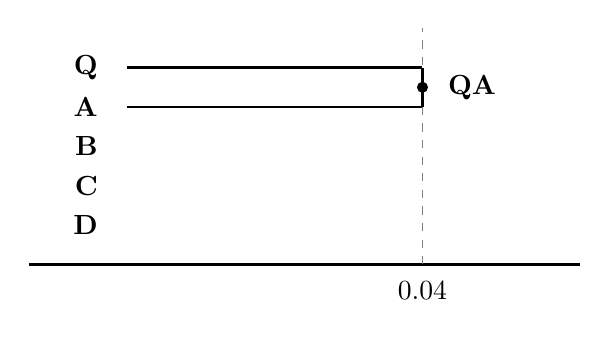
\begin{tikzpicture}
    
        % Axis
        \draw[thick] (-1,-0.5) -- (6,-0.5);
        \draw[dashed, gray] (4,-0.5) -- (4,2.5);
        \node[below] at (4,-0.6) {0.04};
        
        % Labels on the left
        \node[anchor=east] at (0,2) {\textbf{Q}};
        \node[anchor=east] at (0,1.5) {\textbf{A}};
        \node[anchor=east] at (0,1) {\textbf{B}};
        \node[anchor=east] at (0,0.5) {\textbf{C}};
        \node[anchor=east] at (0,0) {\textbf{D}};
        
        % Horizontal lines from labels
        \draw[thick] (0.25,2) -- (4,2);
        \draw[thick] (0.25,1.5) -- (4,1.5);
        
        % Vertical connecting line
        \draw[thick] (4,2) -- (4,1.5);
        
        % Dot at intersection
        \fill (4,1.75) circle (2pt);
        \node[right] at (4.2,1.75) {\textbf{QA}};
        
        \end{tikzpicture}    
    \end{center}
    The branch lengths for A and Q are half the distance between A and Q ($0.08/2 = 0.04$).
    
    \pagebreak
    \textbf{2. Compute matrix D2 with updated distances from QA to remaining proteins B,C,D}
    
    In order to iterate and identify the shortest distance between nodes QA, B, C and D (4 nodes) we need to compute the new distance matrix D2. We always use the original D matrix as the basis to compute distances between individual single proteins. To compute the distance between already clustered nodes (nodes with >1 protein), we compute the mean distance between all possible protein pairs between the two nodes.
    For example: To compute the distance between QAB and CD, we would take the mean between all node distances of QAB and CD as follows
    \begin{equation}
        d_j(QAB, CD) = \frac{d_j(Q, C) + d_j(Q, D) + d_j(A, C) + d_j(A, D) + d_j(B, C) + d_j(B, D)}{6}
    \end{equation}
    This would be the distance between nodes QAB and CD. This is just an example, and you need to find out what proteins will be joined in the next step (which proteins will be joined next) by computing the distance matrix D2 (having nodes QA, B, C, D; so it will be of size $4 \times 4$).

    \textbf{3. Repeat}

    Repeat the joining of the proteins and nodes by computing a new distance matrix at each step (D2, D3, D4) and selecting the closest nodes until you reach the “root” node (QABCD). Draw the tree with all the distances.

    *\underline{Optional task}: Write a complete Python script to compute a UPGMA tree from any number of sequences with the Jaccard measure.
    
\end{question}
\pagebreak
\begin{question}[subtitle = UPGMA computation and visualization with MAFFT web server]
    In this exercise you will use \href{https://mafft.cbrc.jp/alignment/server/}{the MAFFT webserver} to create phylogenetic trees for the original MSF-1 proteins and visualize them.

    \textbf{Part 1:} Conversion of the FASTA file using Python

    In order to interpret our results more easily, we will first change the sequence identifiers to contain only the taxonomic names of each bacterial species. This information is already included in the sequence identifiers and is based on information from \href{https://www.ncbi.nlm.nih.gov/taxonomy}{the NCBO taxonomy database} 

    \underline{Task:} Write a python script that modifies the aligned FASTA file \texttt{mfs\_domain\_proteins.fa} from the previous session to replace the header of each sequence with its taxonomic name. For UniProt headers, this name always follows the \textbf{OS=} prefix (field OrganismName) as defined in the FASTA specification (\url{https://www.uniprot.org/help/fasta-headers}).

    Example:

    \begin{codeblock}
        \texttt{\textgreater$|$A0A017H5R7$|$A0A017H5R7\_9FUSO Acylglycerophosphoethanolamine acyltransferase OS=Fusobacterium necrophorum subsp. funduliforme B35 OX=1226633 GN=FNF\_06146 PE=4 SV=1}\\
        \texttt{MLLTQRKFLPLFLTQFLGALNDNLLKMAIITFITYHLQGSLTEKGILISSVNVITILPMF}\\
        \texttt{FISATAGQFADKFQRNSLVKIIKGIEILGIFFCIFFFYSGQYSLILLTLFVMSTRSAFFG} \\
        \texttt{...}
    \end{codeblock}

    to

    \begin{codeblock}
        \texttt{\textgreater Fusobacterium necrophorum subsp. funduliforme B35}\\
        \texttt{MLLTQRKFLPLFLTQFLGALNDNLLKMAIITFITYHLQGSLTEKGILISSVNVITILPMF}\\
        \texttt{FISATAGQFADKFQRNSLVKIIKGIEILGIFFCIFFFYSGQYSLILLTLFVMSTRSAFFG} \\
        \texttt{...}
    \end{codeblock}
    \small{\textit{Hint: the \texttt{.split()} function can split strings not only on single characters, but also on whole substrings (including “OS=” and ”OX=” !)}}
    \pagebreak
    
    \textbf{Part 2:} Creating a UPGMA tree with MAFFT web server

    Import the modified FASTA file into MAFFT web server. The platform will use MAFFT, an alternative multiple sequence alignment software tool (similar to Clustal Omega), to automatically align the input sequences for you. It offers a stunning range of alignment options, but we are content with leaving these at their default values. You can just click “Submit” and wait for your alignment results.
    After a short while, a page similar ot this should show up:
    
    \begin{figure}[h!]
        \centering
        
\includegraphics[width=1\linewidth]{mafft_webserver.png}
        \label{fig:enter-label}
    \end{figure}
    
    At the bottom of this page you can see the full multiple sequence alignment that MAFFT generated. This MSA will be used as the input for the phylogenetic tree computation in the next step. In order to proceed, now click the button “Phylogenetic tree”. MAFFT web server will offer you many options to fine-tune tree computations. However, in this exercise we are only interested in the “Method” parameter, which lets you select the algorithm to use. Select the option for UPGMA and click “Go!” to compute your tree.

    \textbf{Part 3:} Tree visualization with MAFFT web server

    The next window will offer you a number of ways to visualize and download the resulting tree. Click the “View tree on "Phylo.io" button to reveal the final tree structure.
    
    \underline{Task:} Take a bit of time to inspect the tree: How many major clades (distinct sub-trees) can you see? Which clade features, on average, the most distantly related members? What information do the taxonomic labels provide with regards to the taxonomic hierarchy?
\end{question}

\begin{question}[subtitle=Tree building with the neighborjoining algorithm]
    Another, more frequently used algorithm for phylogenetic tree computation is Neighbor Joining (NJ, proposed by Saitou and Nei in 1987).

    \underline{Task:} Try to repeat exercise 3 by selecting NJ as your clustering algorithm (using only conserved sites). You can then either use a new window or utilize the “Compare” tab in the Phylo.io tree viewer to compare the NJ tree to the previous UPGMA tree. Can you identify clear differences between the trees? From an evolutionary perspective, what do these differences imply? What is the most important algorithmic difference between NJ and UPGMA? (Wikipedia is your friend ;-))

    
\end{question}

\end{document}